\documentclass[
  12pt,
  % handout,
  aspectratio=169
]{beamer}

\usefonttheme{professionalfonts}

\mode<handout> {
  \usepackage{pgfpages}
  \pgfpagesuselayout{4 on 1}[a4paper, landscape]
}

\usepackage[english]{babel}
\usepackage[T1]{fontenc}
\usepackage{lmodern,amsmath,amssymb,alltt,mathtools}
\usepackage{xcolor,colortbl}
\usepackage{xspace}
\usepackage[normalem]{ulem}
\usepackage{verbatim}

\usepackage{tikz}
\usetikzlibrary{arrows,arrows.meta,positioning}

\usepackage{listings}

\definecolor{codegreen}{rgb}{0,0.6,0}
\definecolor{codegray}{rgb}{0.5,0.5,0.5}
\definecolor{codepurple}{rgb}{0.58,0,0.82}

% color scheme
\definecolor{green}{rgb}{0.0,0.5,0.0}
\definecolor{blue}{rgb}{0.0,0.0,0.7}
\definecolor{red}{rgb}{0.8,0.0,0.0}
\definecolor{lightred}{rgb}{1.0,0.97,0.97}
\definecolor{lightblue}{rgb}{0.95,0.95,1.0}
\definecolor{darkblue}{rgb}{0.3,0.3,0.5}
\definecolor{darkred}{rgb}{0.6,0.0,0.0}
\definecolor{darkorange}{rgb}{0.6,0.2,0.1}
\definecolor{darkgreen}{rgb}{0,0.3,0}
%
\newcommand<>{\caution}[1]{\textcolor#2{magenta}{#1}}
\newcommand<>{\cautionblue}[1]{\textcolor#2{blue}{#1}}
\newcommand<>{\strong}[1]{\textcolor#2{blue}{#1}}
\newcommand<>{\h}[1]{\textcolor#2{blue}{#1}}
\newcommand<>{\STRONG}[1]{\textcolor#2{blue}{\bfseries #1}}
\newcommand<>{\CAUTION}[1]{\textcolor#2{magenta}{\bfseries #1}}
\newcommand<>{\ALERT}[1]{\alert#2{\bfseries #1}}
\newcommand{\IMAGE}[2]{\pgfdeclareimage[#1]{#2}{#2}\pgfuseimage{#2}}

\setbeamerfont{title}{series=\bfseries,size=\Large}
\setbeamercolor{title}{fg=red}
\setbeamerfont{subtitle}{series=\bfseries,size=\LARGE}
\setbeamercolor{subtitle}{fg=red}
\setbeamerfont{author}{series=\bfseries,size=\large}
\setbeamercolor{author}{fg=blue}
\setbeamerfont{institute}{series=\bfseries,size=\large}
\setbeamercolor{institute}{fg=green}

\setbeamertemplate{blocks}[rounded]
\setbeamerfont{block title}{series=\bfseries,family=\sffamily,size=\small\strut}
\setbeamercolor{block title}{bg=darkblue,fg=white}
\setbeamercolor{block body}{bg=lightblue}
%\setbeamercolor{block title}{bg=white,fg=darkblue}
%\setbeamercolor{block body}{bg=white}
\setbeamercolor{block title alerted}{bg=darkred,fg=white}
\setbeamercolor{block body alerted}{bg=lightred}
\setbeamercolor{structure}{fg=darkred}
% no fading effect
\makeatletter
\pgfdeclareverticalshading[lower.bg,upper.bg]{bmb@transition}{200cm}{%
  color (0pt)= (lower.bg); color (4pt)= (lower.bg); color (4pt)= (upper.bg)}
\makeatother

% for coding
\newcommand{\kw}[1]{\textcolor{magenta}{\texttt{#1}}}
\newcommand{\idf}[1]{\textcolor{cyan}{\texttt{#1}}}
\newcommand{\cmt}[1]{\textcolor{codegreen}{\texttt{#1}}}
\newcommand{\s}{\texttt{\ }}
\newcommand{\idt}{\mbox{\texttt{\ \ \ \ }}}
\newcommand{\n}[1]{\textcolor{black}{\texttt{#1}}}


\lstdefinestyle{mystyle}{
    commentstyle=\color{codegreen},
    keywordstyle=\color{magenta},
    numberstyle=\tiny\color{codegray},
    stringstyle=\color{codepurple},
    basicstyle=\ttfamily\footnotesize,
    breakatwhitespace=false,
    breaklines=true,
    captionpos=b,
    keepspaces=true,
    numbers=left,
    numbersep=10pt,
    showspaces=false,
    showstringspaces=false,
    showtabs=false,
    tabsize=2
}

\lstset{style=mystyle}


% frametitle
\useframetitletemplate{
\begin{centering}
\centerline{\large\bfseries\color{darkblue}\insertframetitle}
\end{centering}
}

% footer  (title  page/pages)
\setbeamertemplate{navigation symbols}{}
\useheadtemplate{\vbox{\vskip8pt}}
\usefoottemplate{\vbox{\vskip2pt\inserttitle\hfil\insertframenumber/\inserttotalframenumber\vskip5pt}}


% enumerate/itemize environment
\newcommand*\tikzboxed[1]{\tikz[baseline= (c.base)]{%
\node[thick,shape=rectangle,draw,inner sep=2pt] (c) {#1};}}
\setbeamertemplate{items}[square]
\setbeamertemplate{enumerate item}{\tikzboxed{\footnotesize\insertenumlabel}}
\setlength{\itemsep}{1ex}

\title{Four Steps to Conquer Dynamic Programming}
\author{Li Hanyuan}
\date{June 17, 2021}

\begin{document}
\maketitle

\begin{frame}
  \frametitle{Example: Fibonacci Numbers}
  \onslide<+->
  \[
    \mathsf{fib}(n) =
    \begin{cases}
      0 & \text{if } n = 0 \\
      1 & \text{if } n = 1 \\
      \mathsf{fib}(n-1) + \mathsf{fib}(n-2) &
      \text{if } n \geq 2
    \end{cases}
  \]
  \onslide<+->
  \begin{center}
    \begin{minipage}{.5\linewidth}
      % \lstinputlisting[language=python]{fib1.py}
      \kw{def}\s\idf{fib}\n{(n):}\\
      \idt\kw{if}\s\n{n == 0:}\\
      \idt\idt\kw{return}\s\n{0}\\
      \idt\kw{if}\s\n{n == 1:}\\
      \idt\idt\kw{return}\s\n{1}\\
      \idt\kw{return}\s\idf{fib}\n{(n-1)}\n{ + }\idf{fib}\n{(n-2)}
    \end{minipage}
  \end{center}
\end{frame}

\begin{frame}
  \frametitle{Analyzing Complexity}
  \onslide<1,2>
  \centering
  \begin{tikzpicture}
    \node (fib5) at (0,0) {$\mathsf{fib}(5)$};
    \node (fib4) at (-2,-1) {$\mathsf{fib}(4)$};
    \draw (fib5) -- (fib4);
    \node (fib3) at (-4,-2) {$\mathsf{fib}(3)$};
    \draw (fib4) -- (fib3);
    \node (fib2) at (-6,-3) {$\mathsf{fib}(2)$};
    \draw (fib3) -- (fib2);
    \node (fib1) at (-8,-4) {$\mathsf{fib}(1)$};
    \draw (fib2) -- (fib1);

    \node (fib0) at (-5.5,-4) {$\mathsf{fib}(0)$};
    \draw (fib2) -- (fib0);

    \node (fic1) at (-3.5,-3) {$\mathsf{fib}(1)$};
    \draw (fib3) -- (fic1);

    \node (fic2) at (-1,-2) {$\mathsf{fib}(2)$};
    \draw (fib4) -- (fic2);

    \textcolor<handout>{codegray}{
    \onslide<-1>{
    \node (fid1) at (-2,-3) {$\mathsf{fib}(1)$};
    \draw (fic2) -- (fid1);
    \node (fid0) at (-.5,-3) {$\mathsf{fib}(0)$};
    \draw (fic2) -- (fid0);
    }}

    \node (fic3) at (2,-1) {$\mathsf{fib}(3)$};
    \draw (fib5) -- (fic3);

    \textcolor<handout>{codegray}{
    \onslide<-1>{
    \node (fid2) at (1.5,-2) {$\mathsf{fib}(2)$};
    \draw (fic3) -- (fid2);
    \node (fie1) at (1,-3) {$\mathsf{fib}(1)$};
    \draw (fid2) -- (fie1);
    \node (fif1) at (4,-2) {$\mathsf{fib}(1)$};
    \draw (fic3) -- (fif1);
    }}

    \node[right] (tc) at (-3, -4.5) {\textbf{Time Complexity: }};
    \node[right] (sc) at (-3, -5) {\textbf{Space Complexity: }};

    \node[right] (tc1) at (1.5,-4.5) {$O(2^n)$};
    % Why fibonacci recursion is 2^n time complexity?
    % a complete binary tree up to 2^n nodes
    \node[right] at (1.5,-5) {$O(n)$};

    \onslide<2->{

    \node[right] (tc2) at (3.5,-4.5) {$O(n)$};
    \draw [->] (tc1) -- (tc2);

    }

  \end{tikzpicture}
\end{frame}

\begin{frame}
  \frametitle{Optimization: Cache all results}
  \begin{center}
    \begin{minipage}{.5\linewidth}
      \lstinputlisting[language=python]{fib2.py}
    \end{minipage}
  \end{center}
\end{frame}

\begin{frame}
  \frametitle{Top-Down and Bottom-Up}
  \centering
  \onslide<1->
  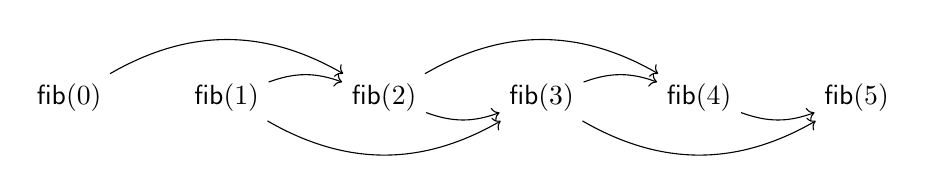
\begin{tikzpicture}
    \onslide<2->{
      \node (fib5) at (10,0) {$\mathsf{fib}(5)$};
    }

    \onslide<4->{
      \node (fib4) at (8, 0) {$\mathsf{fib}(4)$};
      \node (fib3) at (6, 0) {$\mathsf{fib}(3)$};
      \draw [->] (fib3) to[bend right=30] (fib5);
      \draw [->] (fib4) to[bend right=20] (fib5);
    }

    \onslide<5->{
      \node (fib2) at (4, 0) {$\mathsf{fib}(2)$};
      \draw [->] (fib2) to[bend  left=30] (fib4);
      \draw [->] (fib3) to[bend  left=20] (fib4);
    }

    \onslide<6->{
      \node (fib1) at (2, 0) {$\mathsf{fib}(1)$};
      \draw [->] (fib1) to[bend right=30] (fib3);
      \draw [->] (fib2) to[bend right=20] (fib3);
    }

    \onslide<7->{
      \node (fib0) at (0, 0) {$\mathsf{fib}(0)$};
      \draw [->] (fib0) to[bend  left=30] (fib2);
      \draw [->] (fib1) to[bend  left=20] (fib2);
    }

  \end{tikzpicture}
  \vfill
  \begin{columns}
    \begin{column}{0.7\textwidth}
      \null\hfill
      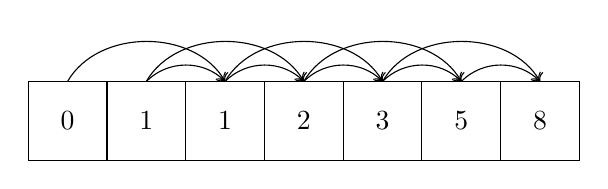
\begin{tikzpicture}
        \onslide<8->{
          \draw (0,0) rectangle (1,1) node at (0.5,0.5) {$0$};
          \draw (1,0) rectangle (2,1) node at (1.5,0.5) {$1$};
        }

        \onslide<9->{
          \draw (2,0) rectangle (3,1) node at (2.5,0.5) {$1$};
        }
        \onslide<9|handout:0>{
          \draw [->] (0.5,1) to[bend left=60] (2.5,1);
          \draw [->] (1.5,1) to[bend left=45] (2.5,1);
        }

        \onslide<10->{
          \draw (3,0) rectangle (4,1) node at (3.5,0.5) {$2$};
        }
        \onslide<10|handout:0>{
          \draw [->] (1.5,1) to[bend left=60] (3.5,1);
          \draw [->] (2.5,1) to[bend left=45] (3.5,1);
        }

        \onslide<11->{
          \draw (4,0) rectangle (5,1) node at (4.5,0.5) {$3$};
        }
        \onslide<11|handout:0>{
          \draw [->] (2.5,1) to[bend left=60] (4.5,1);
          \draw [->] (3.5,1) to[bend left=45] (4.5,1);
        }


        \onslide<12->{
          \draw (5,0) rectangle (6,1) node at (5.5,0.5) {$5$};
        }
        \onslide<12|handout:1>{
          \draw [->] (3.5,1) to[bend left=60] (5.5,1);
          \draw [->] (4.5,1) to[bend left=45] (5.5,1);
        }

        \onslide<13->{
          \draw (6,0) rectangle (7,1) node at (6.5,0.5) {$8$};
        }
        \onslide<13|handout:0>{
          \draw [->] (4.5,1) to[bend left=60] (6.5,1);
          \draw [->] (5.5,1) to[bend left=45] (6.5,1);
        }
      \end{tikzpicture}
      \hspace{2em}
    \end{column}
    \begin{column}{0.3\textwidth}
      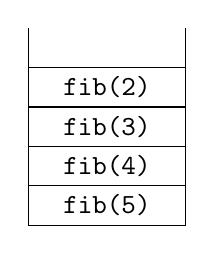
\begin{tikzpicture}
        \onslide<3-7>{
          \draw (0,2.5) -- (0,0) -- (2,0) -- (2,2.5);
        }
        \onslide<3-7>{
          \draw (0,0.5) -- (2,0.5);
          \node at (1,0.25) {\texttt{fib(5)}};
        }
        \onslide<5-7>{
          \draw (0,1.0) -- (2,1.0);
          \node at (1,0.75) {\texttt{fib(4)}};
        }
        \onslide<6-7>{
          \draw (0,1.5) -- (2,1.5);
          \node at (1,1.25) {\texttt{fib(3)}};
        }
        \onslide<7-7>{
          \draw (0,2.0) -- (2,2.0);
          \node at (1,1.75) {\texttt{fib(2)}};
        }
      \end{tikzpicture}
    \end{column}
  \end{columns}

\end{frame}

\begin{frame}
  \frametitle{Optimization: Bottom-Up Cached Table}
  \begin{center}
    \begin{minipage}{.7\linewidth}
      % \lstinputlisting[language=python]{fib3.py}
      \kw{def}\s\idf{fib\_dynamic\_prog}\n{(n):}\\
      \idt\cmt{\# allocate n+1 size cache table}\\
      \idt\n{dp = [0] * (n+1)}\\
      \idt\n{dp[0] = 0; dp[1] = 1}\\
      \idt\kw{for}\s\n{i}\s\kw{in}\s\idf{range}\n{(2, n+1):}\\
      \idt\idt\n{dp[i] = dp[i-1] + dp[i-2]}\\
      \idt\kw{return}\s\n{dp[n]}
    \end{minipage}
  \end{center}
\end{frame}

\begin{frame}
  \frametitle{Optimization: Shrink Space}
  \centering
  \begin{tikzpicture}
    \onslide<1->{
      \textcolor<3-6,9->{codegray}{
        \draw (0,0) rectangle (1,1) node at (0.5,0.5) {$0$};
      }
      \textcolor<4-6,10->{codegray}{
        \draw (1,0) rectangle (2,1) node at (1.5,0.5) {$1$};
      }
    }

    \onslide<2-6,8->{
      \textcolor<5-6,11->{codegray}{
        \draw (2,0) rectangle (3,1) node at (2.5,0.5) {$1$};
      }
    }
    \onslide<2,8|handout:0>{
      \draw [->] (0.5,1) to[bend left=60] (2.5,1);
      \draw [->] (1.5,1) to[bend left=45] (2.5,1);
    }

    \onslide<3-6,9->{
      \textcolor<6,12->{codegray}{
        \draw (3,0) rectangle (4,1) node at (3.5,0.5) {$2$};
      }
    }
    \onslide<3,9|handout:0>{
      \draw [->] (1.5,1) to[bend left=60] (3.5,1);
      \draw [->] (2.5,1) to[bend left=45] (3.5,1);
    }

    \onslide<4-6,10->{
      \draw (4,0) rectangle (5,1) node at (4.5,0.5) {$3$};
    }
    \onslide<4,10|handout:0>{
      \draw [->] (2.5,1) to[bend left=60] (4.5,1);
      \draw [->] (3.5,1) to[bend left=45] (4.5,1);
    }


    \onslide<5-6,11->{
      \draw (5,0) rectangle (6,1) node at (5.5,0.5) {$5$};
    }
    \onslide<5,11|handout:0>{
      \draw [->] (3.5,1) to[bend left=60] (5.5,1);
      \draw [->] (4.5,1) to[bend left=45] (5.5,1);
    }

    \onslide<6,12->{
      \draw (6,0) rectangle (7,1) node at (6.5,0.5) {$8$};
    }
    \onslide<6,12-|handout:1>{
      \draw [->] (4.5,1) to[bend left=60] (6.5,1);
      \draw [->] (5.5,1) to[bend left=45] (6.5,1);
    }

    \onslide<7,8|handout:0>{
      \node (a0) at (0.5, -.5) {$a$};
      \node (b0) at (1.5, -.5) {$b$};
    }

    \onslide<8|handout:0>{
      \node (c0) at (1.5, -1.) {$a'$};
      \node (d0) at (2.5, -1.) {$b'$};
      \draw [->] (a0) -- (c0);
      \draw [->] (b0) -- (d0);
    }

    \onslide<9|handout:0>{
      \node (a1) at (1.5, -0.5) {$a$};
      \node (b1) at (2.5, -0.5) {$b$};
      \node (c1) at (2.5, -1.) {$a'$};
      \node (d1) at (3.5, -1.) {$b'$};
      \draw [->] (a1) -- (c1);
      \draw [->] (b1) -- (d1);
    }

    \onslide<10|handout:0>{
      \node (a2) at (2.5, -0.5) {$a$};
      \node (b2) at (3.5, -0.5) {$b$};
      \node (c2) at (3.5, -1.) {$a'$};
      \node (d2) at (4.5, -1.) {$b'$};
      \draw [->] (a2) -- (c2);
      \draw [->] (b2) -- (d2);
    }

    \onslide<11|handout:0>{
      \node (a3) at (3.5, -0.5) {$a$};
      \node (b3) at (4.5, -0.5) {$b$};
      \node (c3) at (4.5, -1.) {$a'$};
      \node (d3) at (5.5, -1.) {$b'$};
      \draw [->] (a3) -- (c3);
      \draw [->] (b3) -- (d3);
    }

    \onslide<12-|handout:1>{
      \node (a4) at (4.5, -0.5) {$a$};
      \node (b4) at (5.5, -0.5) {$b$};
      \node (c4) at (5.5, -1.) {$a'$};
      \node (d4) at (6.5, -1.) {$b'$};
      \draw [->] (a4) -- (c4);
      \draw [->] (b4) -- (d4);
    }
  \end{tikzpicture}
  \null\vfill
  \begin{minipage}{.5\linewidth}
    \onslide<13->{
      \lstinputlisting[language=python]{fib4.py}
    }
  \end{minipage}
\end{frame}

\begin{frame}
  \frametitle{Four Steps for Dynamic Programming Problems}
  \centering
  \begin{minipage}{.5\linewidth}
    \begin{enumerate}
      \setlength{\itemsep}{1em}
      \item Make recursive solution
      \item Memorization
      \item Make DP table
      \item Shrink space complexity
    \end{enumerate}
  \end{minipage}
\end{frame}

\begin{frame}
  \frametitle{Next Example: Longest Common Subsequence}
  Giving two strings \texttt{text1} and \texttt{text2}, \\
  return the length of their \textbf{longest common subsequence}. \\
  If there is no \textbf{common subsequence},
  return 0. \null\vfill
  \begin{center}
    \begin{tabular}{@{}c@{\hspace{4em}}c@{\hspace{4em}}l@{}}
      \onslide<2->{\large
        \h<5>{B}%
        \h<3,6>{C}%
        \h<3,4,6>{D}%
        \h<3,4,5>{A}%
        \h<3,6>{A}%
        \h<3,4,5,6>{C}%
        \h<3>{D} } &
      \onslide<7->{\large
        A%
        \h<10>{C}%
        \h<8,10>{D}%
        \h<9>{B}%
        \h<8,9,10>{A}%
        \h<8,9,10>{C} }& \vspace{1em}\\
      \onslide<3->{CDAACD} && \\
      \onslide<4->{DAC} & \onslide<8->{DAC} & \onslide<8->{\STRONG{common subsequence}} \\
      \onslide<5->{BAC} & \onslide<9->{BAC} & \onslide<9->{\STRONG{common subsequence}} \\
      \onslide<6->{CDAC} & \onslide<10->{CDAC} & \onslide<10->{\ALERT{longest common subsequence}}
    \end{tabular}
  \end{center}
\end{frame}

\renewcommand{\idt}{\mbox{\texttt{\ \ }}}

\begin{frame}
  \frametitle{Brute Force: Search All Subsequences}
  \onslide<+->
  Iterate all subsequences of each string and find longest common one.

  \onslide<+->
  \textbf{Time Complexity: } $O(2^{n} \times 2^{n}) = O(4^{n})$

  \textbf{Space Complexity: } $O(n)$

  \null\vfill

  \onslide<+->
  \begin{columns}
    \small
    \begin{column}{0.5\textwidth}
      \kw{def}\s\idf{seqs}\n{(arr):}\\
      \idt\kw{if}\s\idf{len}\n{(arr) == 0:}\\
      \idt\idt\kw{yield}\s\n{[]}\\
      \idt\idt\kw{return}\\
      \idt\kw{for}\s\n{subseq}\s\kw{in}\s\idf{seqs}\n{(arr[1:]):}\\
      \idt\idt\kw{yield}\s\n{subseq}\\
      \idt\idt\kw{yield}\s\n{[arr[0], *subseq]}
    \end{column}
    \begin{column}{0.5\textwidth}
      \kw{def}\s\idf{lcs}\n{(text1, text2):}\\
      \idt\n{ans = 0}\\
      \idt\kw{for}\s\n{s1}\s\kw{in}\s\idf{seqs}\n{(text1):}\\
      \idt\idt\kw{for}\s\n{s2}\s\kw{in}\s\idf{seqs}\n{(text2):}\\
      \idt\idt\idt\kw{if}\s\n{s1 == s2:}\\
      \idt\idt\idt\idt\n{ans}\n{ = }\idf{max}\n{(ans, }\idf{len}\n{(s1))}\\
      \idt\kw{return}\s\n{ans}
    \end{column}
  \end{columns}

\end{frame}

\renewcommand{\idt}{\mbox{\texttt{\ \ \ \ }}}

\begin{frame}
  \frametitle{Step1: Make Recursion Solution}
  \begin{columns}
    \begin{column}{.5\textwidth}
      \hfill
      \begin{tikzpicture}
        \only<1-4>{%
          \def\mvu{0}%
          \def\mvd{0}%
        }%
        \only<5>{%
          \def\mvu{0}%
          \def\mvd{-.5}%
        }%
        \only<6>{%
          \def\mvu{-.5}%
          \def\mvd{0}%
        }%
        \only<7>{%
          \def\mvu{-.5}%
          \def\mvd{-.5}%
        }%
        \only<8>{%
          \def\mvu{-1}%
          \def\mvd{-1}%
        }%
        \node at (4,0) {\phantom{.}};
        \foreach \i\c in {0/B,1/C,2/D,3/A,4/A,5/C,6/D} {%
          \node at (\mvu+0.5*\i, 0) {\texttt{\c}};
        }
        \foreach \i\c in {0/A,1/C,2/D,3/B,4/A,5/C} {%
          \node at (\mvd+0.5*\i, -.5) {\texttt{\c}};
        }
        
        \draw (-.2,-.25) rectangle (.2,.25);
        \draw (-.2,-.25) rectangle (.2,-.75);
      \end{tikzpicture}
    \end{column}
    \begin{column}{.5\textwidth}
      \onslide<3->{%
        \texttt{rec(i,j)} means length of\\
        longest common subsequences of strings \\
        \texttt{text1[i:]} and \texttt{text2[j:]}
      }
    \end{column}
  \end{columns}
  \null\vfill
  \begin{columns}
    \begin{column}{.4\textwidth}
      \hfill
      \begin{tabular}{r@{}c@{\quad}c@{\quad}}
        & \texttt{text1[i:]} & \texttt{text2[j:]} \\
        % only if they are same character
        & \ALERT{pick} & \ALERT{pick} \\
        & \CAUTION{drop} & \ALERT{\only<1|handout:0>{pick}\only<2->{?}} \\
        & \ALERT{\only<1|handout:0>{pick}\only<2->{?}} & \CAUTION{drop} \\
        & \onslide<1|handout:0>{\CAUTION{drop}} & \onslide<1|handout:0>{\CAUTION{drop}}
      \end{tabular}
    \end{column}
    \begin{column}{.6\textwidth}
      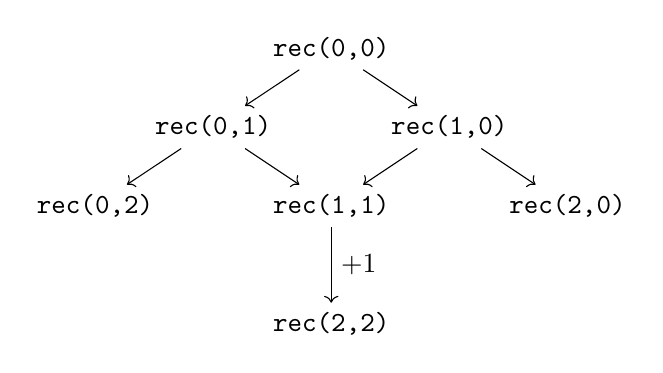
\begin{tikzpicture}
        \onslide<3->{%
          \node (r00) at (0,0) {\texttt{rec(0,0)}};
        }

        \onslide<4->{%
          \node (r01) at (-1.5,-1) {\texttt{rec(0,1)}};
          \node (r10) at (1.5, -1) {\texttt{rec(1,0)}};
          \draw [->] (r00) -- (r01);
          \draw [->] (r00) -- (r10);
        }

        \onslide<5->{%
          \node (r02) at (-3,-2) {\texttt{rec(0,2)}};
          \node (r11) at (0, -2) {\texttt{rec(1,1)}};
          \draw [->] (r01) -- (r02);
          \draw [->] (r01) -- (r11);
        }

        \onslide<6->{%
          \node (r20) at (3, -2) {\texttt{rec(2,0)}};
          \draw [->] (r10) -- (r11);
          \draw [->] (r10) -- (r20);
        }

        \onslide<8->{
          \node (r22) at (0, -3.5) {\texttt{rec(2,2)}};
          \draw [->] (r11) to [edge label={+1}] (r22);
        }
      \end{tikzpicture}
    \end{column}
  \end{columns}
\end{frame}

\begin{frame}
  \centering
  \begin{minipage}{.8\linewidth}
    \onslide<2->{\kw{from}\s\n{functools}\s\kw{import}\s\n{lru\_cache}}\\
    \\
    \kw{def}\s\idf{lcs}\n{(text1, text2):}\\
    \\
    \idt\onslide<2->{\idf{@lru\_cache}\n{(None)}}\\
    \idt\kw{def}\s\idf{rec}\n{(i, j):}\\
    \idt\idt\kw{if}\s\n{i}\s\n{==}\s\idf{len}\n{(text1)}\s\kw{or}\s\n{j}\s\n{==}\s\idf{len}\n{(text2):}\\
    \idt\idt\idt\kw{return}\s\n{0}\\
    \idt\idt\kw{if}\s\n{text1[i] == text2[j]:}\\
    \idt\idt\idt\kw{return}\s\n{1 + }\idf{rec}\n{(i+1, j+1)}\\
    \idt\idt\kw{return}\s\idf{max}\n{(}\\
    \idt\idt\idt\idf{rec}\n{(i, j+1),}\\
    \idt\idt\idt\idf{rec}\n{(i+1, j) )}\\
    \\
    \idt\kw{return}\s\idf{rec}\n{(0, 0)}
  \end{minipage}
\end{frame}

\renewcommand{\idt}{\mbox{\texttt{\ \ }}}

\begin{frame}
  \frametitle{Step 3: Make DP Table}
  \begin{columns}
    \begin{column}{.5\textwidth}
      \centering
      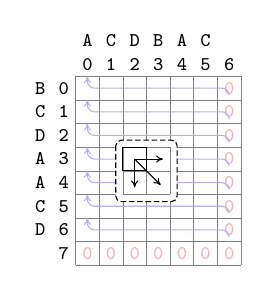
\begin{tikzpicture}
        \def\s{0.3}%
        \draw [help lines, step=\s] (0,0) grid[] (\s*7,\s*-8);
        \scriptsize
        \foreach \i\c in {0/B,1/C,2/D,3/A,4/A,5/C,6/D,7/{}} {%
          \node at (-1.5*\s, -\s*\i-0.5*\s) {\texttt{\c}};
          \node at (-.5*\s, -\s*\i-0.5*\s) {\texttt{\i}};
        }
        \foreach \i\c in {0/A,1/C,2/D,3/B,4/A,5/C,6/{}} {%
          \node at (\s*\i+0.5*\s, 1.5*\s) {\texttt{\c}};
          \node at (\s*\i+0.5*\s, .5*\s) {\texttt{\i}};
        }

        \tikzset{smallarr/.style={arrows = {->[scale width=0.5]}}}%

        \onslide<4->{%
          \foreach \i in {0,...,6} {%
            \node[text=red!30] at (\i*\s+0.5*\s,-7.5*\s) {\texttt{0}};
            \node[text=red!30] at (6.5*\s,-\i*\s-0.5*\s) {\texttt{0}};
          }
        }

        \onslide<3->{%
          \foreach \i in {0,...,6} {%
            \draw [smallarr,draw=blue!30] (6.5*\s,-\i*\s-.8*\s) to[bend right=45] (6.2*\s,-\i*\s-.5*\s) to (0.8*\s,-\i*\s-.5*\s) to[bend left=45] (0.5*\s,-\i*\s-.2*\s) to (0.5*\s,-\i*\s);
          }
        }

        \onslide<2->{%
          \draw[fill=white, rounded corners=2pt, dash pattern=on 2pt off 1pt]
          (1.7*\s, -2.7*\s) rectangle (4.3*\s, -5.3*\s);
          \draw[help lines, step=\s] (\s*2,-3*\s) grid[] (\s*4,-5*\s);
          \draw (2*\s,-3*\s) rectangle (3*\s,-4*\s);
          \draw[smallarr] (2.5*\s,-3.5*\s) to (3.7*\s,-3.5*\s);
          \draw[smallarr] (2.5*\s,-3.5*\s) to (2.5*\s,-4.7*\s);
          \draw[smallarr] (2.5*\s,-3.5*\s) to (3.6*\s,-4.6*\s);
        }
      \end{tikzpicture}
      \null\vspace{1em}
      \onslide<2->
      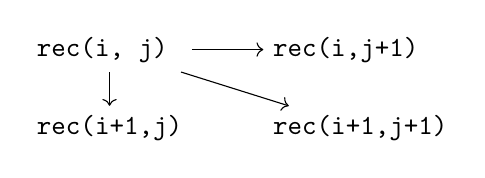
\begin{tikzpicture}
        \node[anchor=west] (r00) at (0,0) {\texttt{rec(i, j)\mbox{\ }}};
        \node[anchor=west] (r01) at (3,0) {\texttt{rec(i,j+1)}};
        \node[anchor=west] (r10) at (0,-1) {\texttt{rec(i+1,j)}};
        \node[anchor=west] (r11) at (3,-1) {\texttt{rec(i+1,j+1)}};
        \draw[->] (r00) -- (r01);
        \draw[->] (r00) -- (r10);
        \draw[->] (r00) -- (r11);
      \end{tikzpicture}
    \end{column}
    \onslide<5->
    \begin{column}{.5\textwidth}
      \scriptsize%
      \kw{def}\s\idf{lcs}\n{(text1, text2):}\\
      \idt\n{dp = [[ 0}\\
      \idt\idt\s\kw{for}\n{ j }\kw{in}\s\idf{range}\n{(}\idf{len}\n{(text2)+1) ]}\\
      \idt\idt\kw{for}\n{ i }\kw{in}\s\idf{range}\n{(}\idf{len}\n{(text1)+1) ]}\\
      \idt\kw{for}\n{ i }\kw{in}\s\idf{range}\n{(}\idf{len}\n{(text1), -1, -1):}\\
      \idt\idt\kw{for}\n{ j }\kw{in}\s\idf{range}\n{(}\idf{len}\n{(text2), -1, -1):}\\
      \idt\idt\idt\kw{if}\s\n{text1[i] == text2[j]:}\\
      \idt\idt\idt\idt\n{dp[i][j] = 1 + dp[i+1][j+1]}\\
      \idt\idt\idt\kw{else}\n{:}\\
      \idt\idt\idt\idt\n{dp[i][j] = }\idf{max}\n{(}\\
      \idt\idt\idt\idt\idt\n{dp[i][j+1],}\\
      \idt\idt\idt\idt\idt\n{dp[i+1][j] )}\\
      \idt\kw{return}\s\n{dp[0][0]}
    \end{column}
  \end{columns}
\end{frame}

\renewcommand{\idt}{\mbox{\texttt{\ \ \ \ }}}

\begin{frame}
  \frametitle{Step 4: Shrink Space Complexity}
  \onslide<+->
  \begin{columns}
    \begin{column}{0.6\textwidth}
      \hfill
      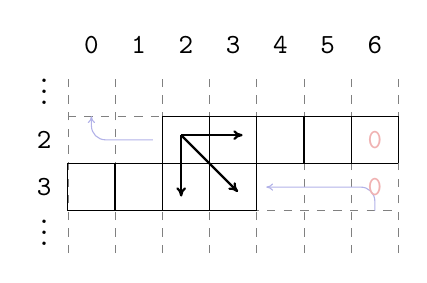
\begin{tikzpicture}[scale=0.6]
        \tikzset{smallarr/.style={arrows = {->[scale width=0.5]}}}%
        \draw [help lines, dashed] (0, 0.9) grid (7, -2.9);
        \foreach \i in {0,...,6} {%
          \node at (0.5+\i,1.5) {\texttt{\i}};
        }
        \foreach \i in {2,...,3} {%
          \node at (-0.5,1.5-\i) {\texttt{\i}};
        }
        \node at (-0.5,.7) {\texttt{\vdots}};
        \node at (-0.5,-2.3) {\texttt{\vdots}};

        \draw (0, -1) grid (4, -2);
        \draw (2, 0) grid (7, -1);

        \draw[smallarr,draw=blue!30] (6.5, -2) to (6.5, -1.8) to[bend right=45] (6.2, -1.5) to (4.2, -1.5);
        \draw[smallarr,draw=blue!30] (1.8, -0.5) to (0.8, -0.5) to[bend left=45] (0.5, -0.2) to (0.5, 0);
        \foreach \i in {2,...,3} {%
          \node[text=red!30] at (6.5,1.5-\i) {\texttt{0}};
        }

        \draw[smallarr, thick] (2.4,-0.4) to (3.7,-0.4);
        \draw[smallarr, thick] (2.4,-0.4) to (2.4,-1.7);
        \draw[smallarr, thick] (2.4,-0.4) to (3.6,-1.6);
      \end{tikzpicture}
      \hspace{2em}
    \end{column}
    \begin{column}{0.4\textwidth}
      \begin{tabular}{|c|c|}
        \hline
        new \texttt{dp[j]} & \texttt{dp[j+1]} \\ \hline
        old \texttt{dp[j]} & \texttt{diag} \\ \hline
      \end{tabular}
      \hfill
    \end{column}
  \end{columns}
  \null\vfill
  \onslide<+->
  \centering
  \begin{minipage}{.4\linewidth}
    \scriptsize%
    \n{dp = [0] * (len(text2) + 1)}\\
    \n{\dots}\\
    \idt\n{newdiag = dp[j]}\\
    \idt\kw{if}\s\n{text1[i] == text2[j]:}\\
    \idt\idt\n{dp[j] = 1 + diag}\\
    \idt\kw{else}\n{:}\\
    \idt\idt\n{dp[j] = max(dp[j], dp[j+1])}\\
    \idt\n{diag = newdiag}\\
    \n{\dots}
  \end{minipage}
\end{frame}

\begin{frame}
  \centering
  \begin{minipage}{.5\linewidth}
    \begin{enumerate}
      \item Make recursive solution
      \item Memorization \\
        \onslide<2->{\ALERT{DO NOT Skip first two steps!}}
      \item Make DP table
      \item Shrink space complexity
    \end{enumerate}
  \end{minipage} \\
  \vspace{3em}
  \onslide<3->
  \begin{minipage}{.6\linewidth}
    \textit{Premature optimization is the root of all evil.} \vspace{1em} \\
    \rightline{{\rm --- Donald Knuth}}
  \end{minipage}
\end{frame}

\end{document}
